\documentclass[tikz]{standalone}
\usepackage{pgfplots}
\pgfplotsset{compat=1.15}
\usepackage{mathrsfs}
\usetikzlibrary{arrows,calc}
\usepackage{tkz-euclide}
\pagestyle{empty}

\definecolor{AngleClr}{rgb}{0,0.39215686274509803,0}
\definecolor{ShapeClr}{rgb}{0.6,0.2,0}

\begin{document}

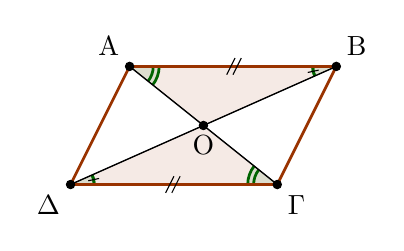
\begin{tikzpicture}[scale=.75]
\tkzSetUpLine[line width=1pt,color=black]
\tkzSetUpPoint[fill=black]

\tkzDefPoints{0/0/D,3.5/0/C,1/2/A,4.5/2/B}

\tkzInterLL(A,C)(B,D) \tkzGetPoint{O}


\tkzFillPolygon[fill=ShapeClr,fill opacity=0.1](A,B,O)
\tkzFillPolygon[fill=ShapeClr,fill opacity=0.1](D,O,C)

\tkzFillAngles[fill=AngleClr,size=.4,fill opacity=0.1](A,B,D C,D,B)
\tkzMarkAngles[line width=1pt,color=AngleClr,size=.4](A,B,D C,D,B)
\tkzMarkAngles[mark=|,mksize=2,line width=1pt,size=.4,color=AngleClr](A,B,D C,D,B)

\tkzFillAngles[fill=AngleClr,size=.5,fill opacity=0.1](O,C,D O,A,B)
\tkzMarkAngles[line width=1pt,color=AngleClr,size=.4](O,C,D O,A,B)
\tkzMarkAngles[line width=1pt,color=AngleClr,size=.5](O,C,D O,A,B)

\tkzDrawSegments[line width=0.5pt,color=black](A,C B,D)

\tkzDrawPolygon[color=ShapeClr](A,B,C,D)
\tkzDrawPoints[size=3](A,B,C,D,O)
\tkzLabelPoint[above left](A){$\rm A$}
\tkzLabelPoint[above right](B){$\rm B$}
\tkzLabelPoint[below right](C){$\rm \Gamma$};
\tkzLabelPoint[below left](D){$\rm \Delta$};
\tkzLabelPoint[below](O){$\rm O$};

\tkzMarkSegments[mark=s||,size=3](C,D A,B)

\end{tikzpicture}
\end{document}
